\documentclass[11pt,a4paper]{article}
\usepackage[margin=2.2cm]{geometry}
\usepackage{lmodern}
\usepackage[T1]{fontenc}
\usepackage{microtype}
\usepackage{amsmath,amssymb,amsthm,bm,mathtools}
\usepackage{booktabs,array}
\usepackage[dvipsnames]{xcolor}
\usepackage[most]{tcolorbox}
\usepackage{tikz}
\usetikzlibrary{arrows.meta}
\usepackage{enumitem}
\usepackage[colorlinks=true,linkcolor=MidnightBlue,urlcolor=MidnightBlue]{hyperref}
\setlength{\parskip}{4pt}\setlength{\parindent}{0pt}
\setlist{itemsep=2pt,topsep=3pt}

\newtcolorbox{plainbox}{colback=blue!4,colframe=MidnightBlue,title=In plain words,fonttitle=\bfseries\small,boxrule=0.6pt,arc=2pt,breakable}
\newtcolorbox{watchbox}{colback=orange!6,colframe=BurntOrange,title=Watch out,fonttitle=\bfseries\small,boxrule=0.6pt,arc=2pt,breakable}
\newtcolorbox{oursbox}{colback=green!5,colframe=ForestGreen,title=What this means for our swarm,fonttitle=\bfseries\small,boxrule=0.6pt,arc=2pt,breakable}
\newtcolorbox{examplebox}{colback=gray!6,colframe=gray!60,title=Worked example,fonttitle=\bfseries\small,boxrule=0.6pt,arc=2pt,breakable}
\newtcolorbox{whybox}{colback=violet!4,colframe=violet!60!black,title=Why it is true,fonttitle=\bfseries\small,boxrule=0.6pt,arc=2pt,breakable}
\newtcolorbox{algbox}[1][]{colback=white,colframe=black!50,title={#1},fonttitle=\bfseries\small,boxrule=0.6pt,arc=2pt,breakable}
\newtcolorbox{testbox}{colback=yellow!7,colframe=olive!70!black,title=How to check your code,fonttitle=\bfseries\small,boxrule=0.6pt,arc=2pt,breakable}

\newcommand{\vect}[1]{\mathbf{#1}}
\newcommand{\R}{\mathbb{R}}
\newcommand{\x}{\vect{x}}
\newcommand{\w}{\vect{w}}
\newcommand{\g}{\vect{g}}

\definecolor{spot}{HTML}{2a78d6}
\definecolor{drone}{HTML}{eb6834}
\definecolor{cellfill}{HTML}{cde2fb}
\tikzset{lat/.style={draw=spot!55,line width=0.5pt}, node/.style={fill=spot}}

\title{\textbf{Self-organising maps, step by step}\\[3pt]
\large What they are, where they came from, how they are trained,\\
and whether they belong in the whoop swarm}
\date{Written for the GNSS-denied whoop swarm project, November 2026}

\begin{document}
\maketitle
\vspace{-1em}
\begin{center}
\begin{minipage}{0.9\textwidth}\small
\textbf{How to read this.} Sections 1--4 explain the self-organising map (SOM): the idea, the parts, the training
rule and what the rule really computes. Section 5 places it in its family, from the 1940s to deep learning today.
Section 6 lists where it is used. Section 7 asks the question that matters for us: does a SOM help the Deformable
Virtual Structure? It includes a small experiment. Section 8 tests the idea of wrapping a SOM around the ground
to locate a drone. The boxes are the same as in the DVS guide: \emph{In plain
words}, \emph{Why it is true}, \emph{Worked example}, \emph{Watch out}, and \emph{How to check your code}.
Section~4 links directly to the Lloyd algorithm we already use.
\end{minipage}
\end{center}

\tableofcontents
\vspace{1em}

%==========================================================================================
\section{The idea in one picture}

A self-organising map is a set of \textbf{units} (also called neurons or nodes) arranged on a fixed grid, the
\textbf{lattice}. Each unit also has a position in the space of the data, its \textbf{prototype} (or weight
vector). Training moves the prototypes so that
\begin{enumerate}[leftmargin=*]
\item every data point has a prototype close to it, and
\item units that are \emph{neighbours on the lattice} end up with prototypes that are \emph{close in the data space}.
\end{enumerate}

\begin{plainbox}
Picture a fishing net. The knots are the units, and the strings are the lattice: which knot is tied to which never
changes. Throw the net over a cloud of points and pull each knot towards the points near it. Because the knots are
tied together, a knot that moves drags its neighbours along. In the end the net is spread over the cloud, and knots
that are neighbours in the net sit near each other in the cloud. The net is a flat, ordered ``map'' of the data.
\end{plainbox}

The idea comes from the brain. In the visual cortex, neighbouring neurons respond to neighbouring points of the
retina, and in the touch area, neighbouring neurons respond to neighbouring patches of skin. Nobody wires these maps
by hand: they organise themselves from experience. Kohonen's SOM (1982) is a simple mathematical model of how such
an ordered map can form.

\begin{center}
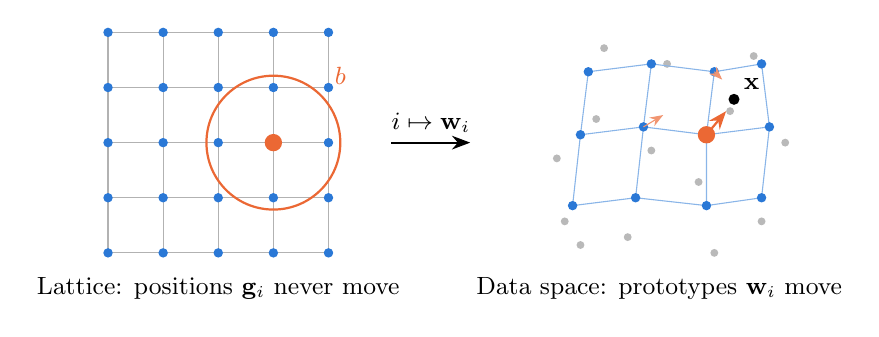
\begin{tikzpicture}[scale=1.0,>=Stealth]
\begin{scope}
  \foreach \i in {0,...,4}{\draw[gray!60] (\i*0.7,0) -- (\i*0.7,2.8); \draw[gray!60] (0,\i*0.7) -- (2.8,\i*0.7);}
  \foreach \i in {0,...,4}{\foreach \j in {0,...,4}{\fill[spot] (\i*0.7,\j*0.7) circle (0.06);}}
  \fill[drone] (2.1,1.4) circle (0.11);
  \draw[drone,thick] (2.1,1.4) circle (0.85);
  \node at (1.4,-0.45) {\small Lattice: positions $\g_i$ never move};
  \node[drone] at (2.95,2.25) {\small $b$};
\end{scope}
\draw[->,thick] (3.6,1.4) -- (4.6,1.4) node[midway,above] {\small $i\mapsto\w_i$};
\begin{scope}[xshift=5.3cm,yshift=-0.2cm]
  \foreach \p in {(0.5,0.6),(0.9,1.9),(1.3,0.4),(1.8,2.6),(2.2,1.1),(2.6,2.0),(3.0,0.6),(1.0,2.8),(0.4,1.4),(2.9,2.7),(1.6,1.5),(3.3,1.6),(0.7,0.3),(2.4,0.2)}{\fill[gray!55] \p circle (0.05);}
  \draw[spot!55] (0.6,0.8) -- (1.4,0.9) -- (2.3,0.8) -- (3.0,0.9);
  \draw[spot!55] (0.7,1.7) -- (1.5,1.8) -- (2.3,1.7) -- (3.1,1.8);
  \draw[spot!55] (0.8,2.5) -- (1.6,2.6) -- (2.4,2.5) -- (3.0,2.6);
  \draw[spot!55] (0.6,0.8) -- (0.7,1.7) -- (0.8,2.5);
  \draw[spot!55] (1.4,0.9) -- (1.5,1.8) -- (1.6,2.6);
  \draw[spot!55] (2.3,0.8) -- (2.3,1.7) -- (2.4,2.5);
  \draw[spot!55] (3.0,0.9) -- (3.1,1.8) -- (3.0,2.6);
  \foreach \p in {(0.6,0.8),(1.4,0.9),(2.3,0.8),(3.0,0.9),(0.7,1.7),(1.5,1.8),(0.8,2.5),(1.6,2.6),(2.4,2.5),(3.0,2.6),(3.1,1.8)}{\fill[spot] \p circle (0.06);}
  \fill[drone] (2.3,1.7) circle (0.11);
  \fill[black] (2.65,2.15) circle (0.07) node[above right] {\small $\x$};
  \draw[->,drone,thick] (2.3,1.7) -- (2.55,2.0);
  \draw[->,drone!70,thin] (1.5,1.8) -- (1.75,1.95);
  \draw[->,drone!70,thin] (2.4,2.5) -- (2.5,2.4);
  \node at (1.7,-0.25) {\small Data space: prototypes $\w_i$ move};
\end{scope}
\end{tikzpicture}\\
\small Left: the lattice. The orange unit $b$ is the best match for the input, and the orange circle is its
neighbourhood. Right: the prototypes in the data space (grey dots are data). The best match moves most towards the
input $\x$; its lattice neighbours move a little, in the same direction.
\end{center}

%==========================================================================================
\section{The parts}

\begin{center}\small
\begin{tabular}{@{}p{3.2cm}p{11.4cm}@{}}
\toprule
Symbol & Meaning\\
\midrule
$\x\in\R^d$ & one data point (an input). The data set is $\x_1,\dots,\x_N$.\\
$i=1,\dots,K$ & the units.\\
$\g_i$ & position of unit $i$ on the lattice (for a $5\times5$ grid: $(0,0),(0,1),\dots,(4,4)$). Fixed forever.\\
$\w_i\in\R^d$ & prototype of unit $i$: where it sits in the data space. This is what training changes.\\
$b(\x)$ & the \textbf{best-matching unit} (BMU, the ``winner''): the unit whose prototype is nearest to $\x$.\\
$h_{bi}$ & the \textbf{neighbourhood function}: how strongly unit $i$ follows when $b$ wins.\\
$\sigma(t)$ & the neighbourhood width, measured in lattice steps. Shrinks during training.\\
$\eta(t)$ & the learning rate, between 0 and 1. Shrinks during training.\\
\bottomrule
\end{tabular}
\end{center}

\textbf{Best-matching unit.}
\begin{equation}
b(\x)=\arg\min_i\ \|\x-\w_i\|^2 .
\end{equation}
This is a competition in the \emph{data} space. It is exactly ``which Voronoi cell of the prototypes contains $\x$''.

\textbf{Neighbourhood function.} It is measured on the \emph{lattice}, not in the data space. The usual choice is a
Gaussian:
\begin{equation}
h_{bi}(t)=\exp\!\Big(-\frac{\|\g_b-\g_i\|^2}{2\,\sigma(t)^2}\Big).
\end{equation}
$h_{bb}=1$ for the winner itself, and $h$ falls off for units further away on the grid. A cheaper alternative is the
``bubble'': $h=1$ inside radius $\sigma$, $0$ outside.

\begin{center}
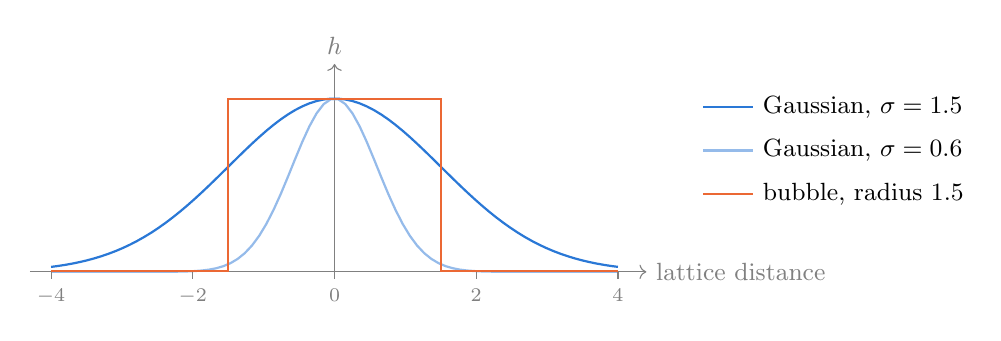
\begin{tikzpicture}[xscale=0.9,yscale=2.2]
  \draw[->,gray] (-4.3,0) -- (4.4,0) node[right] {\small lattice distance};
  \draw[->,gray] (0,0) -- (0,1.2) node[above] {\small $h$};
  \draw[spot,thick,domain=-4:4,samples=80] plot (\x,{exp(-\x*\x/(2*1.5*1.5))});
  \draw[spot!50,thick,domain=-4:4,samples=80] plot (\x,{exp(-\x*\x/(2*0.6*0.6))});
  \draw[drone,thick] (-4,0.004) -- (-1.5,0.004) -- (-1.5,1) -- (1.5,1) -- (1.5,0.004) -- (4,0.004);
  \draw[spot,thick] (5.2,0.95) -- (5.9,0.95) node[right,black] {\small Gaussian, $\sigma=1.5$};
  \draw[spot!50,thick] (5.2,0.7) -- (5.9,0.7) node[right,black] {\small Gaussian, $\sigma=0.6$};
  \draw[drone,thick] (5.2,0.45) -- (5.9,0.45) node[right,black] {\small bubble, radius $1.5$};
  \foreach \t in {-4,-2,0,2,4}{\draw[gray] (\t,0) -- (\t,-0.04) node[below] {\scriptsize $\t$};}
\end{tikzpicture}\\
\small Large $\sigma$: many units move together, so the map is stiff and orders itself globally. Small $\sigma$:
units move almost alone, so they can fit the data finely.
\end{center}

%==========================================================================================
\section{Training}

\subsection{The online rule}
\begin{algbox}[Kohonen's SOM, online version]
\begin{enumerate}[leftmargin=*]
\item Put the prototypes somewhere: random data points, or a flat grid spread along the main directions of the data.
\item Repeat for $t=0,1,\dots,T-1$:
  \begin{enumerate}
  \item pick one data point $\x$ at random;
  \item find the winner $b=\arg\min_i\|\x-\w_i\|^2$;
  \item move \emph{every} unit towards $\x$, each by its own amount:
  \begin{equation}
  \w_i\leftarrow\w_i+\eta(t)\,h_{bi}(t)\,(\x-\w_i)\qquad\text{for all } i ;\label{eq:som}
  \end{equation}
  \item shrink $\eta$ and $\sigma$ a little.
  \end{enumerate}
\end{enumerate}
\end{algbox}

\begin{plainbox}
Equation (\ref{eq:som}) moves unit $i$ a fraction $\eta h_{bi}$ of the way to $\x$. The winner moves the most
($h=1$), its grid neighbours a bit less, and far units hardly at all. With $\eta h=1$ a unit would jump onto
$\x$; with $\eta h=0$ it stays put.
\end{plainbox}

\textbf{Schedules.} A common choice is an exponential decay from a start to an end value:
\[
\eta(t)=\eta_0\Big(\frac{\eta_T}{\eta_0}\Big)^{t/T},\qquad
\sigma(t)=\sigma_0\Big(\frac{\sigma_T}{\sigma_0}\Big)^{t/T}.
\]
Typical values: $\eta_0\approx0.5$, $\eta_T\approx0.01$; $\sigma_0\approx$ half the lattice width, $\sigma_T\approx0.5$
to $1$; $T$ around $500$ times the number of units. Training then has two phases. Early, with large $\sigma$, the map
\textbf{orders} itself: it untangles and takes the rough shape of the data. Late, with small $\sigma$, it
\textbf{converges}: each prototype settles near the data it wins.

\begin{examplebox}
Three units on a chain, so $\g=0,1,2$, with prototypes $\w_1=(0,0)$, $\w_2=(1,0)$, $\w_3=(2,0)$. Input
$\x=(2,1)$, $\eta=0.5$, Gaussian neighbourhood with $\sigma=1$.
\begin{itemize}[leftmargin=*]
\item Squared distances to $\x$: $5,\ 2,\ 1$. The winner is unit 3.
\item Lattice distances from the winner: $2,\ 1,\ 0$, so $h=e^{-2}=0.135,\ e^{-1/2}=0.607,\ 1$.
\item Updates, $\w_i+0.5\,h_i\,(\x-\w_i)$:
\[
\w_3=(2,0)+0.5\cdot1\cdot(0,1)=(2,\ 0.5),
\]
\[
\w_2=(1,0)+0.5\cdot0.607\cdot(1,1)=(1.303,\ 0.303),
\]
\[
\w_1=(0,0)+0.5\cdot0.135\cdot(2,1)=(0.135,\ 0.068).
\]
\end{itemize}
Unit 2 is not the winner, yet it moved almost a third of the way to $\x$, because it is the winner's neighbour on
the chain. That pull is what keeps neighbours together.
\end{examplebox}

\begin{center}
\begin{tikzpicture}[scale=1.25]
\foreach \k/\t/\e in {0/{$t=0$}/{0.560},1/{$t=300$}/{0.414},2/{$t=6000$}/{0.095}}{
\begin{scope}[xshift=\k*2.65cm]
  \fill[gray!8] (0,0) circle (1);
  \draw[gray!60] (0,0) circle (1);
  \input{som_figs/snap\k.tex}
  \node at (0,-1.3) {\small \t};
  \node at (0,-1.62) {\scriptsize mean error \e};
\end{scope}}
\end{tikzpicture}\\
\small An $8\times8$ SOM trained on points spread evenly over a disk. Lines join lattice neighbours. Start: a
small random clump. After 300 steps the map has unfolded into an ordered net. After 6000 it covers the disk, and the
mean distance from a data point to its nearest prototype has dropped from $0.560$ to $0.095$.
\end{center}

\subsection{The batch rule}
Instead of one point at a time, use the whole data set in each round:
\begin{equation}
\w_i\leftarrow\frac{\sum_{n}h_{b(\x_n)\,i}\ \x_n}{\sum_{n}h_{b(\x_n)\,i}} .\label{eq:batch}
\end{equation}
Each prototype becomes a \emph{weighted mean} of the data: points won by unit $i$ count fully, points won by its
lattice neighbours count partly. There is no learning rate, only $\sigma$ shrinks between rounds. The batch rule is
deterministic, often faster, and does not depend on the order of the data.

%==========================================================================================
\section{What the rule really computes}

\subsection{Without neighbours, a SOM is Lloyd's algorithm}
\begin{whybox}
Let $\sigma\to0$. Then $h_{bi}=1$ if $i=b$ and $0$ otherwise. The batch rule (\ref{eq:batch}) becomes
\[
\w_i\leftarrow\frac{\sum_{n:\,b(\x_n)=i}\x_n}{\#\{n:\,b(\x_n)=i\}},
\]
the mean of the points in the Voronoi cell of $\w_i$. That is exactly one round of Lloyd's algorithm (k-means), the
one we use to spread the DVS spots. With samples spread evenly over a shape, the mean of a cell's samples is its
centroid. The online rule with $\sigma\to0$ is the online version of k-means (MacQueen, 1967).
\end{whybox}

So a SOM is \textbf{Lloyd plus a neighbourhood}. The neighbourhood adds one thing Lloyd does not have: an order. Lloyd
treats the spots as an unlabelled set; a SOM keeps track of who is next to whom on a fixed grid.

\subsection{The price of the neighbourhood}
The pull between neighbours never fully disappears while $\sigma>0$. Each prototype is pulled slightly towards its
neighbours' data, so it sits slightly off the centroid of its own cell. Two consequences:
\begin{itemize}[leftmargin=*]
\item The final map covers the data a little worse than plain Lloyd (higher quantisation error).
\item Prototypes near the edge of the data are pulled inwards, so the map shrinks slightly away from the boundary.
\end{itemize}
Ending with a small $\sigma$, or finishing with a few rounds of plain Lloyd, removes most of this.

\subsection{Is there a cost that the SOM minimises?}
Lloyd lowers a clear cost, the total squared distance from points to their nearest spot. The natural guess for a SOM
is the neighbourhood-weighted version
\[
E=\sum_n\sum_i h_{b(\x_n)\,i}\,\|\x_n-\w_i\|^2 .
\]
\begin{watchbox}
The standard SOM rule is \emph{not} exact gradient descent on this or any single cost when the data are continuous
(Erwin, Obermayer and Schulten, 1992). The trouble is the winner: it is chosen by plain distance, which does not
match how $E$ changes. Heskes (1999) showed that changing the winner rule to
$b(\x)=\arg\min_j\sum_i h_{ji}\|\x-\w_i\|^2$ gives a version that does minimise $E$. In practice the standard rule
works well; just do not expect a convergence proof like the one for Lloyd.
\end{watchbox}

\subsection{How to measure a trained map}
\begin{itemize}[leftmargin=*]
\item \textbf{Quantisation error}: the mean distance from each data point to its winner. Small means good coverage.
\item \textbf{Topographic error}: the fraction of data points whose best and second-best units are \emph{not} lattice
neighbours. Small means the order is kept.
\item \textbf{U-matrix}: for each unit, the average data-space distance to its lattice neighbours, drawn as a grey
image on the lattice. Light valleys are clusters; dark ridges are borders between them.
\end{itemize}
The two errors pull against each other: a stiff map (large $\sigma$) keeps order but covers badly, a loose map covers
well but can fold.

%==========================================================================================
\section{The family: ancestors, relatives and modern versions}

\begin{center}
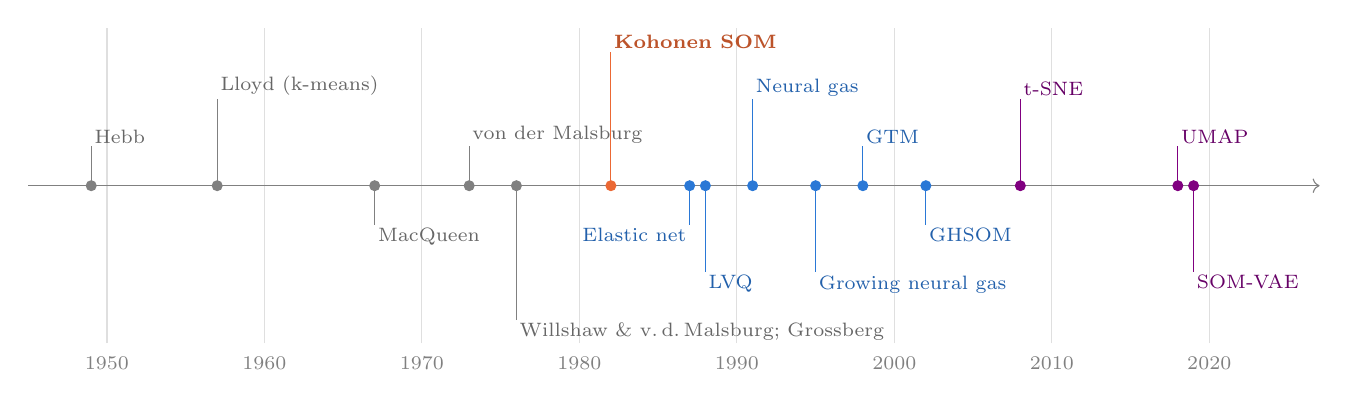
\begin{tikzpicture}[x=0.2cm,y=1cm,font=\scriptsize]
  \foreach \yr in {1950,1960,1970,1980,1990,2000,2010,2020}{
    \draw[gray!25] ({\yr-1945},-2.0) -- ({\yr-1945},2.0);
    \node[gray] at ({\yr-1945},-2.25) {\yr};}
  \draw[->,gray] (0,0) -- (82,0);
  \foreach \yr/\lvl/\name/\c in {
    1949/0.5/Hebb/gray, 1957/1.1/Lloyd (k-means)/gray, 1973/0.5/von der Malsburg/gray,
    1982/1.7/\textbf{Kohonen SOM}/drone, 1991/1.1/Neural gas/spot, 1998/0.5/GTM/spot,
    2008/1.1/t-SNE/violet, 2018/0.5/UMAP/violet}{
    \draw[\c] ({\yr-1945},0) -- ({\yr-1945},\lvl);
    \fill[\c] ({\yr-1945},0) circle (2pt);
    \node[anchor=south west,inner sep=1pt,\c!80!black] at ({\yr-1945},\lvl) {\name};}
  \foreach \yr/\lvl/\name/\c in {
    1967/-0.5/MacQueen/gray, 1976/-1.7/{Willshaw \& v.\,d.\,Malsburg; Grossberg}/gray,
    1988/-1.1/LVQ/spot, 1995/-1.1/Growing neural gas/spot,
    2002/-0.5/GHSOM/spot, 2019/-1.1/SOM-VAE/violet}{
    \draw[\c] ({\yr-1945},0) -- ({\yr-1945},\lvl);
    \fill[\c] ({\yr-1945},0) circle (2pt);
    \node[anchor=north west,inner sep=1pt,\c!80!black] at ({\yr-1945},\lvl) {\name};}
  \draw[spot] (42,0) -- (42,-0.5);
  \fill[spot] (42,0) circle (2pt);
  \node[anchor=north east,inner sep=1pt,spot!80!black] at (42,-0.5) {Elastic net};
\end{tikzpicture}\\
\small Grey: ancestors. Orange: the SOM. Blue: relatives and successors in the same spirit. Violet: modern methods
that took over some of its jobs.
\end{center}

\subsection{Ancestors}
\begin{itemize}[leftmargin=*]
\item \textbf{Hebb (1949)}: ``cells that fire together wire together''. Learning as local strengthening of
connections, the root of every rule of the form ``move the weights towards the input''.
\item \textbf{Lloyd (1957, published 1982) and MacQueen (1967)}: k-means. Prototypes as cell means; the
$\sigma\to0$ limit of the SOM.
\item \textbf{von der Malsburg (1973)}; \textbf{Willshaw and von der Malsburg (1976)}: models of how ordered maps,
such as the map from the retina to the brain, set themselves up through local competition and cooperation.
\item \textbf{Grossberg (1976)}; later \textbf{Rumelhart and Zipser (1985)}: competitive learning, where units compete
for inputs and only the winner learns. The SOM is competitive learning in which the winner shares its update with its
neighbours.
\end{itemize}

\subsection{Relatives and successors}
\begin{center}\small
\begin{tabular}{@{}p{3.6cm}p{11cm}@{}}
\toprule
Method & How it differs from the SOM\\
\midrule
Elastic net (Durbin \& Willshaw, 1987) & A closed 1D chain pulled towards points while its length is penalised. Built
for the travelling salesman problem: the chain becomes the tour.\\
LVQ (Kohonen, about 1988--90) & Supervised: prototypes carry class labels and move towards inputs of their own class,
away from others. No lattice.\\
Neural gas (Martinetz \& Schulten, 1991) & No fixed lattice. Units are ranked by distance to the input and the update
falls off with rank. Neighbours are learned, not given, so it fits data of any shape and dimension.\\
Growing neural gas (Fritzke, 1995) & Starts with two units and adds units where the error is largest, learning the
connections as it goes. Number of units need not be chosen in advance.\\
GTM (Bishop, Svensén \& Williams, 1998) & A probabilistic SOM: a smooth map from a latent grid to the data space,
trained by maximum likelihood (EM). Has a real cost function and gives probabilities.\\
GHSOM (Rauber, Merkl \& Dittenbach, 2002) & A tree of SOMs: each map grows, and units that still cover too much data
get their own child map.\\
\bottomrule
\end{tabular}
\end{center}

\subsection{Modern versions and replacements}
\begin{itemize}[leftmargin=*]
\item \textbf{t-SNE (van der Maaten \& Hinton, 2008)} and \textbf{UMAP (McInnes et al., 2018)} took over the SOM's
most popular job, drawing high-dimensional data in 2D. They place each data point directly instead of fitting a grid,
and usually show clusters more clearly. They do not give a reusable grid of prototypes.
\item \textbf{SOM-VAE (Fortuin et al., 2019)} puts a SOM inside a deep network: a variational autoencoder compresses
the data, and the compressed codes are snapped to SOM nodes, giving discrete states that can be read and followed
over time. Several ``deep SOM'' variants follow the same idea.
\item The SOM itself is still used where a fixed, ordered grid of prototypes is the point: data inspection with
U-matrices, small embedded systems, and as a baseline.
\end{itemize}

%==========================================================================================
\section{Typical applications}
\begin{itemize}[leftmargin=*]
\item \textbf{Exploring and visualising data}: each unit becomes a cell of a 2D picture; similar inputs land in nearby
cells. Used for documents (Kohonen's WEBSOM organised millions of documents), finance, gene expression and sensor
data.
\item \textbf{Clustering and compression}: the prototypes are a codebook (vector quantisation), with the bonus that
nearby codes mean similar things.
\item \textbf{Speech}: Kohonen's ``phonetic typewriter'' (1988) mapped speech sounds onto a 2D map of phonemes.
\item \textbf{Routing}: a closed chain stretched over cities gives a short tour (Angéniol, Vaubois and Le~Texier,
1988; the elastic net). Also used for multi-robot inspection tours.
\item \textbf{Robotics}: learning arm kinematics and hand--eye coordination (Ritter, Martinetz and Schulten, 1989),
and assigning robots to targets in changing environments (Zhu and Yang, 2006).
\item \textbf{Anomaly detection}: a point far from every prototype is unusual.
\end{itemize}

%==========================================================================================
\section{Does a SOM belong in the DVS?}

\subsection{The translation}
\begin{center}\small
\begin{tabular}{@{}p{4.2cm}p{10.4cm}@{}}
\toprule
SOM & DVS\\
\midrule
unit $i$ & drone $i$ (its spot)\\
prototype $\w_i$ & spot $\vect{p}_{i,c}$ in the template\\
data points $\x_n$ & points spread evenly over the template shape\\
lattice $\g_i$ & a fixed grid among the drones, for example their slots on the bench\\
winner & ``which spot is nearest'': the Voronoi cell\\
$\sigma\to0$ & exactly our Lloyd step\\
\bottomrule
\end{tabular}
\end{center}

So a SOM on the template would be our Lloyd step with one extra wish: \emph{drones that are bench neighbours should
end up as formation neighbours}. That wish sounds useful (fewer crossing paths, a stable neighbour graph for the cell
complex), so we tested it.

\subsection{A small experiment}
Sixteen drones on a $4\times4$ bench grid must spread over an L-shaped region (the square $[0,2]^2$ minus the corner
where $x>1$ and $y>1$). The L is not convex and an affine map cannot turn a disk into it, so the DVS shortcut of
``Lloyd once, then map'' does not cover this case. 8000 points sampled evenly over the L stand in for the shape.
\begin{itemize}[leftmargin=*]
\item \textbf{Lloyd + Hungarian} (our current pipeline): seeds from the bench grid, recentred and scaled into the L
with a small nudge, Lloyd on the samples, then the assignment.
\item \textbf{SOM}: the same seeds as starting prototypes, the bench grid as the lattice, $8000$ online steps with
$\sigma$ from $1.5$ to $0.3$ and $\eta$ from $0.4$ to $0.01$.
\end{itemize}
Each was run 5 times with different nudges. ``Pairs kept'' counts how many of the 24 bench-neighbour pairs are still
neighbours in the final layout (neighbours in the Delaunay graph).

\begin{center}\small
\begin{tabular}{@{}lccc@{}}
\toprule
& Pairs kept & Coverage error (mean sq.\ distance) & Closest pair\\
\midrule
Lloyd + Hungarian & $0.93$ & $\mathbf{0.0320}$ & $\mathbf{0.341}$\\
SOM & $0.94$ & $0.0347$ & $0.301$\\
\bottomrule
\end{tabular}
\end{center}

\begin{center}
\begin{tikzpicture}[scale=1.55]
\foreach \k/\name/\lab in {0/lloyd/{Lloyd + Hungarian},1/som/{SOM}}{
\begin{scope}[xshift=\k*3.3cm]
  \fill[gray!8] (0,0) -- (2,0) -- (2,1) -- (1,1) -- (1,2) -- (0,2) -- cycle;
  \draw[gray!60] (0,0) -- (2,0) -- (2,1) -- (1,1) -- (1,2) -- (0,2) -- cycle;
  \input{som_figs/exp_\name.tex}
  \node at (1,-0.3) {\small \lab};
\end{scope}}
\end{tikzpicture}\\
\small One run of each. Lines join drones that were neighbours on the bench. Both keep the bench order almost
everywhere; the SOM pulls its outer drones slightly inwards.
\end{center}

\begin{oursbox}
In this test the SOM bought nothing. Our drone-seeded Lloyd already keeps the bench order (because it starts from
the bench and moves little), and the Hungarian step keeps paths short. The SOM kept about the same number of pairs,
covered the shape about 8\,\% worse, and its closest pair was about 12\,\% closer. The closest pair matters most for
us: the body size is $r=r_0\,l_s/l_{\min}$, so a 12\,\% smaller $l_{\min}$ means a 12\,\% bigger formation for the
same safety distance. This is one shape and five runs, not a proof, but it points one way.
\end{oursbox}

\subsection{Where a SOM could still help}
\begin{itemize}[leftmargin=*]
\item \textbf{Smooth reshaping}. If the template itself changes shape over time (not just move, scale, squish, rotate),
running a few SOM steps per update moves every spot a little, in order, instead of recomputing a fresh layout and
reassigning. That is the elastic-net idea: the formation as a net that stretches to a new shape. Splitting a body into
two, or growing a merged one, are such reshapes.
\item \textbf{A learned controller}. A SOM-like rule (move towards the samples you win, share a little with your grid
neighbours) is local and cheap, which suits drones that decide for themselves. Our plan is centralised, so this does
not apply now.
\item \textbf{Inspection routes}. A closed chain (elastic net) over points of interest gives a short tour for a
group to follow. That is a path-planning use outside the DVS itself.
\end{itemize}

\subsection{Where it does not help}
\begin{itemize}[leftmargin=*]
\item \textbf{Assignment}. For 100 drones or fewer, the Hungarian algorithm gives the exact best matching in
milliseconds. A SOM gives an approximate one.
\item \textbf{Safety}. A SOM has no exact cost and no convergence guarantee (Section 4.3), and it lowers the closest
distance. Our safety chain needs guarantees, so a SOM can only ever propose a layout that is then checked.
\item \textbf{Move, scale, squish, rotate}. These are affine, so the template cells are simply mapped and nothing
needs relearning.
\end{itemize}

\begin{plainbox}
A SOM is Lloyd with a memory of who sits next to whom. For the DVS as it is now, Lloyd seeded from the drones already
gives that memory for free, with better spacing. The interesting place for a SOM is \emph{non-affine reshaping}, for
example during a split or a merge, where it could carry the formation smoothly from one shape to another. That is a
question to test later, against Lloyd + Hungarian, with spacing as the main measure.
\end{plainbox}

%==========================================================================================
\section{Wrapping a SOM around the ground: can it locate a drone?}\label{sec:ground}

\subsection{The idea}
Each drone measures the ground below it: the range sensor gives the distance to the floor, and the bottom camera
gives floor points. Collect these measurements from all drones and let a SOM wrap around them: a 2D net whose
prototypes live in 3D and settle onto the ground surface, including anything standing on it. The net is then a
\textbf{map of the ground}. A drone can compare what it measures now with that map and so work out where it is,
in all three coordinates, without drift.

\begin{plainbox}
Think of feeling your way across a dark room with a walking stick. The stick only tells you how far down the floor
is. On an empty floor that tells you nothing about where you are. But when the stick drops off the edge of a step,
and you have a map of where the steps are, you know where you are. The SOM is one way to draw that map. The real
question is whether the floor has enough ``steps'' to recognise.
\end{plainbox}

\begin{center}
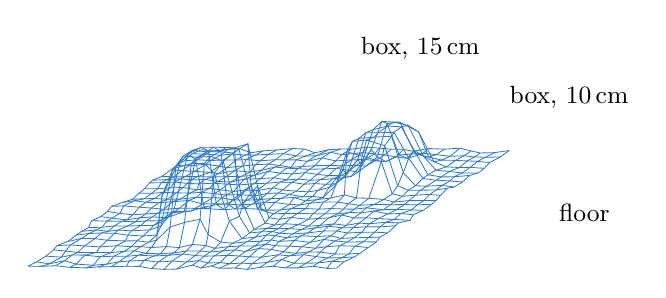
\begin{tikzpicture}[scale=2.1,mesh/.style={draw=spot,line width=0.3pt}]
\draw[mesh] (0.097,0.031) -- (0.148,0.056) -- (0.204,0.091) -- (0.252,0.129) -- (0.272,0.155) -- (0.339,0.180) -- (0.387,0.218) -- (0.422,0.241) -- (0.463,0.264) -- (0.481,0.305) -- (0.536,0.330) -- (0.577,0.361) -- (0.601,0.392) -- (0.670,0.416) -- (0.728,0.435) -- (0.769,0.472) -- (0.801,0.499) -- (0.831,0.534) -- (0.849,0.550) -- (0.907,0.574) -- (0.962,0.614) -- (0.996,0.639) -- (1.039,0.667) -- (1.089,0.710) -- (1.146,0.735);
\draw[mesh] (0.097,0.031) -- (0.174,0.029) -- (0.263,0.033) -- (0.351,0.023) -- (0.450,0.020) -- (0.520,0.026) -- (0.598,0.027) -- (0.691,0.030) -- (0.770,0.029) -- (0.844,0.016) -- (0.919,0.011) -- (0.995,0.013) -- (1.092,0.037) -- (1.142,0.019) -- (1.206,0.032) -- (1.251,0.018) -- (1.349,0.019) -- (1.422,0.011) -- (1.499,0.023) -- (1.579,0.030) -- (1.653,0.020) -- (1.731,0.020) -- (1.820,0.030) -- (1.905,0.017) -- (1.962,0.018);
\draw[mesh] (0.174,0.029) -- (0.227,0.045) -- (0.298,0.085) -- (0.325,0.122) -- (0.353,0.159) -- (0.420,0.198) -- (0.466,0.228) -- (0.513,0.250) -- (0.544,0.266) -- (0.574,0.303) -- (0.604,0.321) -- (0.653,0.350) -- (0.674,0.395) -- (0.741,0.426) -- (0.799,0.438) -- (0.843,0.471) -- (0.880,0.499) -- (0.903,0.535) -- (0.935,0.554) -- (0.980,0.570) -- (1.026,0.608) -- (1.068,0.637) -- (1.122,0.674) -- (1.172,0.708) -- (1.209,0.727);
\draw[mesh] (0.148,0.056) -- (0.227,0.045) -- (0.317,0.063) -- (0.388,0.043) -- (0.491,0.036) -- (0.574,0.043) -- (0.647,0.057) -- (0.709,0.061) -- (0.799,0.066) -- (0.884,0.055) -- (0.969,0.062) -- (1.054,0.055) -- (1.131,0.064) -- (1.185,0.050) -- (1.259,0.052) -- (1.315,0.045) -- (1.389,0.049) -- (1.451,0.045) -- (1.543,0.053) -- (1.630,0.070) -- (1.706,0.048) -- (1.778,0.048) -- (1.850,0.050) -- (1.935,0.060) -- (2.006,0.056);
\draw[mesh] (0.263,0.033) -- (0.317,0.063) -- (0.364,0.098) -- (0.397,0.113) -- (0.439,0.153) -- (0.501,0.197) -- (0.540,0.231) -- (0.579,0.241) -- (0.619,0.274) -- (0.665,0.302) -- (0.692,0.310) -- (0.730,0.341) -- (0.770,0.387) -- (0.809,0.417) -- (0.863,0.440) -- (0.912,0.476) -- (0.957,0.504) -- (0.984,0.539) -- (1.019,0.559) -- (1.046,0.572) -- (1.104,0.604) -- (1.173,0.647) -- (1.199,0.669) -- (1.261,0.701) -- (1.306,0.736);
\draw[mesh] (0.204,0.091) -- (0.298,0.085) -- (0.364,0.098) -- (0.440,0.097) -- (0.534,0.087) -- (0.617,0.091) -- (0.694,0.090) -- (0.764,0.097) -- (0.857,0.092) -- (0.944,0.096) -- (1.032,0.104) -- (1.108,0.095) -- (1.162,0.091) -- (1.221,0.092) -- (1.301,0.096) -- (1.374,0.092) -- (1.435,0.087) -- (1.508,0.085) -- (1.610,0.099) -- (1.679,0.093) -- (1.763,0.100) -- (1.840,0.088) -- (1.907,0.080) -- (1.995,0.082) -- (2.071,0.086);
\draw[mesh] (0.351,0.023) -- (0.388,0.043) -- (0.440,0.097) -- (0.510,0.113) -- (0.532,0.147) -- (0.576,0.187) -- (0.620,0.229) -- (0.642,0.249) -- (0.698,0.273) -- (0.746,0.299) -- (0.774,0.323) -- (0.808,0.346) -- (0.843,0.382) -- (0.887,0.414) -- (0.938,0.435) -- (0.995,0.474) -- (1.034,0.506) -- (1.060,0.531) -- (1.083,0.552) -- (1.120,0.572) -- (1.199,0.598) -- (1.251,0.636) -- (1.280,0.673) -- (1.332,0.709) -- (1.377,0.742);
\draw[mesh] (0.252,0.129) -- (0.325,0.122) -- (0.397,0.113) -- (0.510,0.113) -- (0.598,0.112) -- (0.679,0.121) -- (0.740,0.123) -- (0.810,0.108) -- (0.897,0.105) -- (0.979,0.111) -- (1.054,0.122) -- (1.138,0.122) -- (1.199,0.116) -- (1.276,0.123) -- (1.350,0.129) -- (1.411,0.119) -- (1.490,0.137) -- (1.567,0.132) -- (1.642,0.117) -- (1.718,0.108) -- (1.795,0.117) -- (1.863,0.115) -- (1.954,0.104) -- (2.037,0.104) -- (2.105,0.109);
\draw[mesh] (0.450,0.020) -- (0.491,0.036) -- (0.534,0.087) -- (0.598,0.112) -- (0.632,0.154) -- (0.685,0.183) -- (0.701,0.218) -- (0.722,0.244) -- (0.779,0.276) -- (0.808,0.304) -- (0.848,0.328) -- (0.880,0.351) -- (0.918,0.374) -- (0.969,0.420) -- (1.017,0.436) -- (1.076,0.472) -- (1.118,0.492) -- (1.130,0.528) -- (1.167,0.555) -- (1.212,0.570) -- (1.248,0.590) -- (1.299,0.626) -- (1.354,0.672) -- (1.406,0.702) -- (1.444,0.716);
\draw[mesh] (0.272,0.155) -- (0.353,0.159) -- (0.439,0.153) -- (0.532,0.147) -- (0.632,0.154) -- (0.721,0.148) -- (0.779,0.149) -- (0.843,0.143) -- (0.934,0.149) -- (1.012,0.143) -- (1.091,0.162) -- (1.172,0.155) -- (1.227,0.138) -- (1.306,0.148) -- (1.377,0.152) -- (1.470,0.153) -- (1.536,0.164) -- (1.591,0.154) -- (1.676,0.151) -- (1.751,0.148) -- (1.836,0.139) -- (1.901,0.148) -- (1.981,0.154) -- (2.073,0.151) -- (2.154,0.143);
\draw[mesh] (0.520,0.026) -- (0.574,0.043) -- (0.617,0.091) -- (0.679,0.121) -- (0.721,0.148) -- (0.757,0.184) -- (0.793,0.213) -- (0.833,0.250) -- (0.856,0.277) -- (0.894,0.305) -- (0.936,0.324) -- (0.974,0.354) -- (1.012,0.381) -- (1.071,0.428) -- (1.116,0.447) -- (1.146,0.477) -- (1.195,0.501) -- (1.220,0.532) -- (1.245,0.543) -- (1.297,0.572) -- (1.346,0.608) -- (1.398,0.637) -- (1.416,0.675) -- (1.472,0.703) -- (1.520,0.728);
\draw[mesh] (0.339,0.180) -- (0.420,0.198) -- (0.501,0.197) -- (0.576,0.187) -- (0.685,0.183) -- (0.757,0.184) -- (0.825,0.175) -- (0.874,0.188) -- (0.956,0.267) -- (1.043,0.295) -- (1.137,0.314) -- (1.186,0.221) -- (1.262,0.176) -- (1.334,0.169) -- (1.421,0.178) -- (1.504,0.181) -- (1.567,0.189) -- (1.614,0.180) -- (1.708,0.186) -- (1.802,0.174) -- (1.886,0.192) -- (1.954,0.183) -- (2.026,0.176) -- (2.126,0.178) -- (2.203,0.177);
\draw[mesh] (0.598,0.027) -- (0.647,0.057) -- (0.694,0.090) -- (0.740,0.123) -- (0.779,0.149) -- (0.825,0.175) -- (0.876,0.219) -- (0.900,0.272) -- (0.930,0.311) -- (0.976,0.361) -- (1.041,0.360) -- (1.086,0.365) -- (1.109,0.380) -- (1.152,0.407) -- (1.213,0.444) -- (1.223,0.469) -- (1.260,0.492) -- (1.303,0.526) -- (1.321,0.539) -- (1.387,0.574) -- (1.440,0.600) -- (1.473,0.644) -- (1.502,0.668) -- (1.551,0.707) -- (1.601,0.733);
\draw[mesh] (0.387,0.218) -- (0.466,0.228) -- (0.540,0.231) -- (0.620,0.229) -- (0.701,0.218) -- (0.793,0.213) -- (0.876,0.219) -- (0.907,0.455) -- (0.990,0.624) -- (1.084,0.651) -- (1.163,0.652) -- (1.222,0.592) -- (1.314,0.303) -- (1.391,0.197) -- (1.471,0.206) -- (1.539,0.219) -- (1.590,0.215) -- (1.664,0.202) -- (1.748,0.214) -- (1.846,0.210) -- (1.928,0.214) -- (1.991,0.198) -- (2.068,0.202) -- (2.156,0.204) -- (2.224,0.206);
\draw[mesh] (0.691,0.030) -- (0.709,0.061) -- (0.764,0.097) -- (0.810,0.108) -- (0.843,0.143) -- (0.874,0.188) -- (0.907,0.455) -- (0.969,0.609) -- (1.016,0.659) -- (1.063,0.707) -- (1.110,0.676) -- (1.160,0.387) -- (1.188,0.378) -- (1.225,0.408) -- (1.268,0.443) -- (1.293,0.461) -- (1.340,0.482) -- (1.374,0.522) -- (1.403,0.556) -- (1.467,0.580) -- (1.508,0.610) -- (1.551,0.648) -- (1.593,0.674) -- (1.641,0.711) -- (1.697,0.742);
\draw[mesh] (0.422,0.241) -- (0.513,0.250) -- (0.579,0.241) -- (0.642,0.249) -- (0.722,0.244) -- (0.833,0.250) -- (0.900,0.272) -- (0.969,0.609) -- (1.036,0.697) -- (1.119,0.689) -- (1.203,0.694) -- (1.277,0.664) -- (1.375,0.332) -- (1.437,0.231) -- (1.507,0.238) -- (1.574,0.240) -- (1.618,0.230) -- (1.695,0.225) -- (1.791,0.232) -- (1.885,0.243) -- (1.964,0.243) -- (2.029,0.231) -- (2.115,0.235) -- (2.194,0.236) -- (2.272,0.232);
\draw[mesh] (0.770,0.029) -- (0.799,0.066) -- (0.857,0.092) -- (0.897,0.105) -- (0.934,0.149) -- (0.956,0.267) -- (0.990,0.624) -- (1.036,0.697) -- (1.089,0.730) -- (1.144,0.749) -- (1.187,0.727) -- (1.236,0.403) -- (1.285,0.372) -- (1.313,0.405) -- (1.331,0.432) -- (1.376,0.463) -- (1.407,0.491) -- (1.461,0.529) -- (1.503,0.560) -- (1.548,0.604) -- (1.590,0.630) -- (1.619,0.639) -- (1.660,0.673) -- (1.719,0.697) -- (1.767,0.739);
\draw[mesh] (0.463,0.264) -- (0.544,0.266) -- (0.619,0.274) -- (0.698,0.273) -- (0.779,0.276) -- (0.856,0.277) -- (0.930,0.311) -- (1.016,0.659) -- (1.089,0.730) -- (1.179,0.722) -- (1.256,0.723) -- (1.337,0.715) -- (1.396,0.408) -- (1.464,0.253) -- (1.542,0.259) -- (1.610,0.257) -- (1.675,0.258) -- (1.750,0.252) -- (1.827,0.260) -- (1.912,0.272) -- (1.996,0.263) -- (2.062,0.263) -- (2.140,0.268) -- (2.226,0.268) -- (2.319,0.275);
\draw[mesh] (0.844,0.016) -- (0.884,0.055) -- (0.944,0.096) -- (0.979,0.111) -- (1.012,0.143) -- (1.043,0.295) -- (1.084,0.651) -- (1.119,0.689) -- (1.179,0.722) -- (1.216,0.750) -- (1.262,0.727) -- (1.303,0.408) -- (1.347,0.377) -- (1.385,0.401) -- (1.419,0.429) -- (1.470,0.455) -- (1.481,0.487) -- (1.540,0.532) -- (1.584,0.565) -- (1.622,0.593) -- (1.660,0.623) -- (1.687,0.628) -- (1.719,0.673) -- (1.773,0.696) -- (1.833,0.716);
\draw[mesh] (0.481,0.305) -- (0.574,0.303) -- (0.665,0.302) -- (0.746,0.299) -- (0.808,0.304) -- (0.894,0.305) -- (0.976,0.361) -- (1.063,0.707) -- (1.144,0.749) -- (1.216,0.750) -- (1.296,0.748) -- (1.372,0.739) -- (1.443,0.472) -- (1.531,0.291) -- (1.588,0.279) -- (1.648,0.287) -- (1.733,0.282) -- (1.791,0.272) -- (1.863,0.277) -- (1.948,0.286) -- (2.021,0.277) -- (2.099,0.291) -- (2.161,0.287) -- (2.260,0.296) -- (2.336,0.292);
\draw[mesh] (0.919,0.011) -- (0.969,0.062) -- (1.032,0.104) -- (1.054,0.122) -- (1.091,0.162) -- (1.137,0.314) -- (1.163,0.652) -- (1.203,0.694) -- (1.256,0.723) -- (1.296,0.748) -- (1.346,0.746) -- (1.365,0.442) -- (1.404,0.379) -- (1.451,0.405) -- (1.497,0.433) -- (1.544,0.470) -- (1.577,0.504) -- (1.622,0.539) -- (1.660,0.552) -- (1.693,0.588) -- (1.728,0.620) -- (1.754,0.633) -- (1.785,0.664) -- (1.839,0.698) -- (1.915,0.735);
\draw[mesh] (0.536,0.330) -- (0.604,0.321) -- (0.692,0.310) -- (0.774,0.323) -- (0.848,0.328) -- (0.936,0.324) -- (1.041,0.360) -- (1.110,0.676) -- (1.187,0.727) -- (1.262,0.727) -- (1.346,0.746) -- (1.426,0.770) -- (1.485,0.515) -- (1.554,0.323) -- (1.619,0.314) -- (1.689,0.325) -- (1.792,0.314) -- (1.851,0.319) -- (1.914,0.322) -- (1.994,0.340) -- (2.066,0.322) -- (2.141,0.323) -- (2.214,0.318) -- (2.311,0.313) -- (2.407,0.308);
\draw[mesh] (0.995,0.013) -- (1.054,0.055) -- (1.108,0.095) -- (1.138,0.122) -- (1.172,0.155) -- (1.186,0.221) -- (1.222,0.592) -- (1.277,0.664) -- (1.337,0.715) -- (1.372,0.739) -- (1.426,0.770) -- (1.445,0.517) -- (1.484,0.376) -- (1.529,0.417) -- (1.568,0.439) -- (1.609,0.473) -- (1.637,0.491) -- (1.692,0.537) -- (1.732,0.557) -- (1.773,0.596) -- (1.798,0.616) -- (1.833,0.638) -- (1.874,0.685) -- (1.927,0.719) -- (1.988,0.739);
\draw[mesh] (0.577,0.361) -- (0.653,0.350) -- (0.730,0.341) -- (0.808,0.346) -- (0.880,0.351) -- (0.974,0.354) -- (1.086,0.365) -- (1.160,0.387) -- (1.236,0.403) -- (1.303,0.408) -- (1.365,0.442) -- (1.445,0.517) -- (1.508,0.369) -- (1.581,0.347) -- (1.650,0.349) -- (1.727,0.350) -- (1.819,0.347) -- (1.893,0.347) -- (1.972,0.348) -- (2.041,0.355) -- (2.110,0.353) -- (2.191,0.364) -- (2.272,0.346) -- (2.352,0.349) -- (2.426,0.341);
\draw[mesh] (1.092,0.037) -- (1.131,0.064) -- (1.162,0.091) -- (1.199,0.116) -- (1.227,0.138) -- (1.262,0.176) -- (1.314,0.303) -- (1.375,0.332) -- (1.396,0.408) -- (1.443,0.472) -- (1.485,0.515) -- (1.508,0.369) -- (1.547,0.369) -- (1.588,0.415) -- (1.628,0.441) -- (1.677,0.464) -- (1.720,0.484) -- (1.766,0.526) -- (1.803,0.550) -- (1.845,0.586) -- (1.889,0.619) -- (1.925,0.640) -- (1.958,0.667) -- (1.994,0.705) -- (2.050,0.738);
\draw[mesh] (0.601,0.392) -- (0.674,0.395) -- (0.770,0.387) -- (0.843,0.382) -- (0.918,0.374) -- (1.012,0.381) -- (1.109,0.380) -- (1.188,0.378) -- (1.285,0.372) -- (1.347,0.377) -- (1.404,0.379) -- (1.484,0.376) -- (1.547,0.369) -- (1.623,0.370) -- (1.685,0.378) -- (1.777,0.379) -- (1.856,0.375) -- (1.929,0.379) -- (2.005,0.376) -- (2.069,0.375) -- (2.141,0.383) -- (2.246,0.372) -- (2.326,0.373) -- (2.418,0.371) -- (2.485,0.367);
\draw[mesh] (1.142,0.019) -- (1.185,0.050) -- (1.221,0.092) -- (1.276,0.123) -- (1.306,0.148) -- (1.334,0.169) -- (1.391,0.197) -- (1.437,0.231) -- (1.464,0.253) -- (1.531,0.291) -- (1.554,0.323) -- (1.581,0.347) -- (1.623,0.370) -- (1.678,0.404) -- (1.705,0.446) -- (1.760,0.450) -- (1.791,0.480) -- (1.830,0.530) -- (1.863,0.553) -- (1.914,0.578) -- (1.960,0.622) -- (1.999,0.637) -- (2.051,0.673) -- (2.121,0.717) -- (2.151,0.750);
\draw[mesh] (0.670,0.416) -- (0.741,0.426) -- (0.809,0.417) -- (0.887,0.414) -- (0.969,0.420) -- (1.071,0.428) -- (1.152,0.407) -- (1.225,0.408) -- (1.313,0.405) -- (1.385,0.401) -- (1.451,0.405) -- (1.529,0.417) -- (1.588,0.415) -- (1.678,0.404) -- (1.741,0.401) -- (1.799,0.411) -- (1.883,0.418) -- (1.971,0.418) -- (2.034,0.408) -- (2.101,0.398) -- (2.191,0.404) -- (2.288,0.402) -- (2.373,0.403) -- (2.450,0.401) -- (2.538,0.405);
\draw[mesh] (1.206,0.032) -- (1.259,0.052) -- (1.301,0.096) -- (1.350,0.129) -- (1.377,0.152) -- (1.421,0.178) -- (1.471,0.206) -- (1.507,0.238) -- (1.542,0.259) -- (1.588,0.279) -- (1.619,0.314) -- (1.650,0.349) -- (1.685,0.378) -- (1.741,0.401) -- (1.773,0.425) -- (1.818,0.452) -- (1.848,0.488) -- (1.899,0.525) -- (1.939,0.559) -- (1.991,0.578) -- (2.040,0.609) -- (2.082,0.640) -- (2.135,0.676) -- (2.193,0.710) -- (2.221,0.744);
\draw[mesh] (0.728,0.435) -- (0.799,0.438) -- (0.863,0.440) -- (0.938,0.435) -- (1.017,0.436) -- (1.116,0.447) -- (1.213,0.444) -- (1.268,0.443) -- (1.331,0.432) -- (1.419,0.429) -- (1.497,0.433) -- (1.568,0.439) -- (1.628,0.441) -- (1.705,0.446) -- (1.773,0.425) -- (1.842,0.433) -- (1.928,0.443) -- (2.010,0.461) -- (2.083,0.443) -- (2.158,0.441) -- (2.249,0.434) -- (2.309,0.418) -- (2.400,0.427) -- (2.490,0.427) -- (2.565,0.428);
\draw[mesh] (1.251,0.018) -- (1.315,0.045) -- (1.374,0.092) -- (1.411,0.119) -- (1.470,0.153) -- (1.504,0.181) -- (1.539,0.219) -- (1.574,0.240) -- (1.610,0.257) -- (1.648,0.287) -- (1.689,0.325) -- (1.727,0.350) -- (1.777,0.379) -- (1.799,0.411) -- (1.842,0.433) -- (1.880,0.445) -- (1.917,0.506) -- (1.957,0.529) -- (2.004,0.564) -- (2.051,0.573) -- (2.092,0.599) -- (2.141,0.636) -- (2.197,0.668) -- (2.251,0.703) -- (2.294,0.738);
\draw[mesh] (0.769,0.472) -- (0.843,0.471) -- (0.912,0.476) -- (0.995,0.474) -- (1.076,0.472) -- (1.146,0.477) -- (1.223,0.469) -- (1.293,0.461) -- (1.376,0.463) -- (1.470,0.455) -- (1.544,0.470) -- (1.609,0.473) -- (1.677,0.464) -- (1.760,0.450) -- (1.818,0.452) -- (1.880,0.445) -- (1.957,0.518) -- (2.024,0.722) -- (2.117,0.696) -- (2.233,0.662) -- (2.299,0.468) -- (2.361,0.453) -- (2.440,0.460) -- (2.527,0.464) -- (2.591,0.458);
\draw[mesh] (1.349,0.019) -- (1.389,0.049) -- (1.435,0.087) -- (1.490,0.137) -- (1.536,0.164) -- (1.567,0.189) -- (1.590,0.215) -- (1.618,0.230) -- (1.675,0.258) -- (1.733,0.282) -- (1.792,0.314) -- (1.819,0.347) -- (1.856,0.375) -- (1.883,0.418) -- (1.928,0.443) -- (1.957,0.518) -- (2.000,0.612) -- (2.026,0.588) -- (2.090,0.675) -- (2.112,0.645) -- (2.172,0.736) -- (2.209,0.690) -- (2.261,0.663) -- (2.323,0.691) -- (2.367,0.737);
\draw[mesh] (0.801,0.499) -- (0.880,0.499) -- (0.957,0.504) -- (1.034,0.506) -- (1.118,0.492) -- (1.195,0.501) -- (1.260,0.492) -- (1.340,0.482) -- (1.407,0.491) -- (1.481,0.487) -- (1.577,0.504) -- (1.637,0.491) -- (1.720,0.484) -- (1.791,0.480) -- (1.848,0.488) -- (1.917,0.506) -- (2.000,0.612) -- (2.058,0.785) -- (2.144,0.793) -- (2.253,0.759) -- (2.332,0.517) -- (2.396,0.490) -- (2.469,0.490) -- (2.564,0.491) -- (2.633,0.502);
\draw[mesh] (1.422,0.011) -- (1.451,0.045) -- (1.508,0.085) -- (1.567,0.132) -- (1.591,0.154) -- (1.614,0.180) -- (1.664,0.202) -- (1.695,0.225) -- (1.750,0.252) -- (1.791,0.272) -- (1.851,0.319) -- (1.893,0.347) -- (1.929,0.379) -- (1.971,0.418) -- (2.010,0.461) -- (2.024,0.722) -- (2.058,0.785) -- (2.098,0.803) -- (2.139,0.837) -- (2.184,0.856) -- (2.237,0.906) -- (2.268,0.893) -- (2.341,0.703) -- (2.391,0.682) -- (2.426,0.725);
\draw[mesh] (0.831,0.534) -- (0.903,0.535) -- (0.984,0.539) -- (1.060,0.531) -- (1.130,0.528) -- (1.220,0.532) -- (1.303,0.526) -- (1.374,0.522) -- (1.461,0.529) -- (1.540,0.532) -- (1.622,0.539) -- (1.692,0.537) -- (1.766,0.526) -- (1.830,0.530) -- (1.899,0.525) -- (1.957,0.529) -- (2.026,0.588) -- (2.098,0.803) -- (2.191,0.811) -- (2.295,0.816) -- (2.366,0.596) -- (2.440,0.517) -- (2.508,0.514) -- (2.601,0.519) -- (2.673,0.509);
\draw[mesh] (1.499,0.023) -- (1.543,0.053) -- (1.610,0.099) -- (1.642,0.117) -- (1.676,0.151) -- (1.708,0.186) -- (1.748,0.214) -- (1.791,0.232) -- (1.827,0.260) -- (1.863,0.277) -- (1.914,0.322) -- (1.972,0.348) -- (2.005,0.376) -- (2.034,0.408) -- (2.083,0.443) -- (2.117,0.696) -- (2.144,0.793) -- (2.191,0.811) -- (2.215,0.837) -- (2.271,0.878) -- (2.306,0.902) -- (2.346,0.901) -- (2.437,0.710) -- (2.486,0.713) -- (2.518,0.742);
\draw[mesh] (0.849,0.550) -- (0.935,0.554) -- (1.019,0.559) -- (1.083,0.552) -- (1.167,0.555) -- (1.245,0.543) -- (1.321,0.539) -- (1.403,0.556) -- (1.503,0.560) -- (1.584,0.565) -- (1.660,0.552) -- (1.732,0.557) -- (1.803,0.550) -- (1.863,0.553) -- (1.939,0.559) -- (2.004,0.564) -- (2.090,0.675) -- (2.139,0.837) -- (2.215,0.837) -- (2.310,0.840) -- (2.399,0.683) -- (2.484,0.561) -- (2.564,0.550) -- (2.649,0.546) -- (2.724,0.539);
\draw[mesh] (1.579,0.030) -- (1.630,0.070) -- (1.679,0.093) -- (1.718,0.108) -- (1.751,0.148) -- (1.802,0.174) -- (1.846,0.210) -- (1.885,0.243) -- (1.912,0.272) -- (1.948,0.286) -- (1.994,0.340) -- (2.041,0.355) -- (2.069,0.375) -- (2.101,0.398) -- (2.158,0.441) -- (2.233,0.662) -- (2.253,0.759) -- (2.295,0.816) -- (2.310,0.840) -- (2.354,0.873) -- (2.395,0.882) -- (2.458,0.843) -- (2.519,0.690) -- (2.566,0.705) -- (2.615,0.738);
\draw[mesh] (0.907,0.574) -- (0.980,0.570) -- (1.046,0.572) -- (1.120,0.572) -- (1.212,0.570) -- (1.297,0.572) -- (1.387,0.574) -- (1.467,0.580) -- (1.548,0.604) -- (1.622,0.593) -- (1.693,0.588) -- (1.773,0.596) -- (1.845,0.586) -- (1.914,0.578) -- (1.991,0.578) -- (2.051,0.573) -- (2.112,0.645) -- (2.184,0.856) -- (2.271,0.878) -- (2.354,0.873) -- (2.433,0.730) -- (2.515,0.583) -- (2.596,0.570) -- (2.672,0.571) -- (2.767,0.579);
\draw[mesh] (1.653,0.020) -- (1.706,0.048) -- (1.763,0.100) -- (1.795,0.117) -- (1.836,0.139) -- (1.886,0.192) -- (1.928,0.214) -- (1.964,0.243) -- (1.996,0.263) -- (2.021,0.277) -- (2.066,0.322) -- (2.110,0.353) -- (2.141,0.383) -- (2.191,0.404) -- (2.249,0.434) -- (2.299,0.468) -- (2.332,0.517) -- (2.366,0.596) -- (2.399,0.683) -- (2.433,0.730) -- (2.488,0.695) -- (2.552,0.662) -- (2.599,0.672) -- (2.648,0.695) -- (2.710,0.744);
\draw[mesh] (0.962,0.614) -- (1.026,0.608) -- (1.104,0.604) -- (1.199,0.598) -- (1.248,0.590) -- (1.346,0.608) -- (1.440,0.600) -- (1.508,0.610) -- (1.590,0.630) -- (1.660,0.623) -- (1.728,0.620) -- (1.798,0.616) -- (1.889,0.619) -- (1.960,0.622) -- (2.040,0.609) -- (2.092,0.599) -- (2.172,0.736) -- (2.237,0.906) -- (2.306,0.902) -- (2.395,0.882) -- (2.488,0.695) -- (2.564,0.611) -- (2.645,0.603) -- (2.722,0.594) -- (2.818,0.594);
\draw[mesh] (1.731,0.020) -- (1.778,0.048) -- (1.840,0.088) -- (1.863,0.115) -- (1.901,0.148) -- (1.954,0.183) -- (1.991,0.198) -- (2.029,0.231) -- (2.062,0.263) -- (2.099,0.291) -- (2.141,0.323) -- (2.191,0.364) -- (2.246,0.372) -- (2.288,0.402) -- (2.309,0.418) -- (2.361,0.453) -- (2.396,0.490) -- (2.440,0.517) -- (2.484,0.561) -- (2.515,0.583) -- (2.564,0.611) -- (2.626,0.631) -- (2.683,0.670) -- (2.733,0.698) -- (2.776,0.727);
\draw[mesh] (0.996,0.639) -- (1.068,0.637) -- (1.173,0.647) -- (1.251,0.636) -- (1.299,0.626) -- (1.398,0.637) -- (1.473,0.644) -- (1.551,0.648) -- (1.619,0.639) -- (1.687,0.628) -- (1.754,0.633) -- (1.833,0.638) -- (1.925,0.640) -- (1.999,0.637) -- (2.082,0.640) -- (2.141,0.636) -- (2.209,0.690) -- (2.268,0.893) -- (2.346,0.901) -- (2.458,0.843) -- (2.552,0.662) -- (2.626,0.631) -- (2.706,0.627) -- (2.771,0.628) -- (2.856,0.622);
\draw[mesh] (1.820,0.030) -- (1.850,0.050) -- (1.907,0.080) -- (1.954,0.104) -- (1.981,0.154) -- (2.026,0.176) -- (2.068,0.202) -- (2.115,0.235) -- (2.140,0.268) -- (2.161,0.287) -- (2.214,0.318) -- (2.272,0.346) -- (2.326,0.373) -- (2.373,0.403) -- (2.400,0.427) -- (2.440,0.460) -- (2.469,0.490) -- (2.508,0.514) -- (2.564,0.550) -- (2.596,0.570) -- (2.645,0.603) -- (2.706,0.627) -- (2.753,0.667) -- (2.797,0.691) -- (2.831,0.715);
\draw[mesh] (1.039,0.667) -- (1.122,0.674) -- (1.199,0.669) -- (1.280,0.673) -- (1.354,0.672) -- (1.416,0.675) -- (1.502,0.668) -- (1.593,0.674) -- (1.660,0.673) -- (1.719,0.673) -- (1.785,0.664) -- (1.874,0.685) -- (1.958,0.667) -- (2.051,0.673) -- (2.135,0.676) -- (2.197,0.668) -- (2.261,0.663) -- (2.341,0.703) -- (2.437,0.710) -- (2.519,0.690) -- (2.599,0.672) -- (2.683,0.670) -- (2.753,0.667) -- (2.815,0.664) -- (2.889,0.657);
\draw[mesh] (1.905,0.017) -- (1.935,0.060) -- (1.995,0.082) -- (2.037,0.104) -- (2.073,0.151) -- (2.126,0.178) -- (2.156,0.204) -- (2.194,0.236) -- (2.226,0.268) -- (2.260,0.296) -- (2.311,0.313) -- (2.352,0.349) -- (2.418,0.371) -- (2.450,0.401) -- (2.490,0.427) -- (2.527,0.464) -- (2.564,0.491) -- (2.601,0.519) -- (2.649,0.546) -- (2.672,0.571) -- (2.722,0.594) -- (2.771,0.628) -- (2.815,0.664) -- (2.864,0.689) -- (2.917,0.717);
\draw[mesh] (1.089,0.710) -- (1.172,0.708) -- (1.261,0.701) -- (1.332,0.709) -- (1.406,0.702) -- (1.472,0.703) -- (1.551,0.707) -- (1.641,0.711) -- (1.719,0.697) -- (1.773,0.696) -- (1.839,0.698) -- (1.927,0.719) -- (1.994,0.705) -- (2.121,0.717) -- (2.193,0.710) -- (2.251,0.703) -- (2.323,0.691) -- (2.391,0.682) -- (2.486,0.713) -- (2.566,0.705) -- (2.648,0.695) -- (2.733,0.698) -- (2.797,0.691) -- (2.864,0.689) -- (2.953,0.691);
\draw[mesh] (1.962,0.018) -- (2.006,0.056) -- (2.071,0.086) -- (2.105,0.109) -- (2.154,0.143) -- (2.203,0.177) -- (2.224,0.206) -- (2.272,0.232) -- (2.319,0.275) -- (2.336,0.292) -- (2.407,0.308) -- (2.426,0.341) -- (2.485,0.367) -- (2.538,0.405) -- (2.565,0.428) -- (2.591,0.458) -- (2.633,0.502) -- (2.673,0.509) -- (2.724,0.539) -- (2.767,0.579) -- (2.818,0.594) -- (2.856,0.622) -- (2.889,0.657) -- (2.953,0.691) -- (3.007,0.730);
\draw[mesh] (1.146,0.735) -- (1.209,0.727) -- (1.306,0.736) -- (1.377,0.742) -- (1.444,0.716) -- (1.520,0.728) -- (1.601,0.733) -- (1.697,0.742) -- (1.767,0.739) -- (1.833,0.716) -- (1.915,0.735) -- (1.988,0.739) -- (2.050,0.738) -- (2.151,0.750) -- (2.221,0.744) -- (2.294,0.738) -- (2.367,0.737) -- (2.426,0.725) -- (2.518,0.742) -- (2.615,0.738) -- (2.710,0.744) -- (2.776,0.727) -- (2.831,0.715) -- (2.917,0.717) -- (3.007,0.730);

\node[anchor=west] at (3.25,0.35) {\small floor};
\node[anchor=west] at (2.05,1.35) {\small box, 15\,cm};
\node[anchor=west] at (2.95,1.05) {\small box, 10\,cm};
\end{tikzpicture}\\
\small A $25\times25$ SOM trained on 6000 noisy ground points (1\,cm noise) over a $2\times2$\,m floor with two
boxes, drawn in perspective with height exaggerated. The net settles onto the floor and climbs over the boxes.
\end{center}

\subsection{Step 1: turning measurements into ground points}
A drone at position $(x,y,z)$, tilted by an angle $\beta$ from vertical, measuring range $d$ straight down its own
axis, sees the ground at height
\[
z_g=z-d\cos\beta ,
\]
at roughly the point $(x,y)$ (exactly, the point is shifted sideways by $d\sin\beta$ in the direction of the tilt).
A floor point seen by the camera at pixel offset $(u,v)$ from the image centre, with focal length $f$ in pixels and
height $h$ above the floor, lies at $(x+hu/f,\ y+hv/f)$, using the fixed shared heading. Every reading becomes a 3D
point $(x_g,y_g,z_g)$. The SOM is trained on these points exactly as in Section 3, with $\w_i\in\R^3$.

\subsection{Step 2: locating a drone against the map}
Let $h(x,y)$ be the ground height in the map. A drone flying level at an unknown height $z_0$ measures a sequence
of ranges $d_k$. Its own estimate of where it was, $\hat{\vect{p}}_k$, has drifted by an unknown offset
$\vect{\delta}=(\delta_x,\delta_y)$, so the true positions are $\hat{\vect{p}}_k+\vect{\delta}$. The model is
\[
d_k=z_0-h(\hat{\vect{p}}_k+\vect{\delta})+\text{noise},
\]
and the best offset and height are the ones that explain the readings best:
\begin{equation}
(\hat z_0,\hat{\vect{\delta}})=\arg\min_{z_0,\vect{\delta}}\ \sum_k\big(d_k-z_0+h(\hat{\vect{p}}_k+\vect{\delta})\big)^2 .
\label{eq:match}
\end{equation}
This is \emph{map matching}: slide the recent range profile over the map until it fits.

\subsection{When does it work? The information matrix}
Near the answer, a small change $\Delta\vect{\delta}$ changes each predicted reading by $-\nabla h_k\cdot
\Delta\vect{\delta}$, where $\nabla h_k$ is the slope of the ground under reading $k$. With measurement noise
$\sigma$, the amount of information the readings carry about $\vect{\delta}$ is the matrix
\begin{equation}
\vect{I}=\frac{1}{\sigma^2}\sum_k\nabla h_k\,\nabla h_k^{\!\top}.
\end{equation}
The position can only be found in the directions where $\vect{I}$ is not zero.
\begin{itemize}[leftmargin=*]
\item \textbf{Flat floor:} every slope is zero, so $\vect{I}=\vect{0}$. Nothing about $x,y$ can be learned. Only
the height $z_0$ is found, which the range sensor gives directly anyway.
\item \textbf{One straight edge:} all slopes point across the edge, so every $\nabla h_k\nabla h_k^{\!\top}$ has the
same direction and $\vect{I}$ has rank 1. The position \emph{across} the edge is found, the position \emph{along} it
is not.
\item \textbf{A corner, or two edges at an angle:} slopes in two directions, $\vect{I}$ has rank 2, and both $x$ and
$y$ are found.
\end{itemize}
\begin{whybox}
The matrix $\vect{I}$ is the curvature of the cost (\ref{eq:match}) around its minimum. If $\vect{I}\vect{v}=\vect{0}$
for some direction $\vect{v}$, moving the offset along $\vect{v}$ does not change the cost: the cost has a flat
valley, and every point in it fits equally well. A sum of outer products $\nabla h\nabla h^{\!\top}$ has full rank
only if the slopes $\nabla h_k$ span both directions.
\end{whybox}

\begin{center}
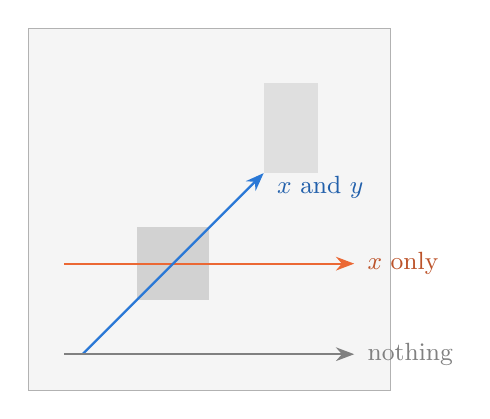
\begin{tikzpicture}[scale=2.3,>=Stealth]
  \fill[gray!8] (0,0) rectangle (2,2);
  \draw[gray!60] (0,0) rectangle (2,2);
  \fill[gray!35] (0.6,0.5) rectangle (1.0,0.9);
  \fill[gray!25] (1.3,1.2) rectangle (1.6,1.7);
  \draw[->,thick,drone] (0.2,0.7) -- (1.8,0.7);
  \node[anchor=west,drone!80!black] at (1.82,0.7) {\small $x$ only};
  \draw[->,thick,spot] (0.3,0.2) -- (1.3,1.2);
  \node[anchor=west,spot!80!black] at (1.32,1.12) {\small $x$ and $y$};
  \draw[->,thick,gray] (0.2,0.2) -- (1.8,0.2);
  \node[anchor=west,gray] at (1.82,0.2) {\small nothing};
\end{tikzpicture}\\
\small Top view of the test floor. Orange: a straight flight across the first box crosses two edges that both run
in $y$, so only $x$ is fixed. Blue: a diagonal flight over a corner crosses edges in both directions. Grey: a flight
over bare floor.
\end{center}

\subsection{A test}
The floor of the figures: $2\times2$\,m with two boxes, 15\,cm and 10\,cm high. Two maps were built from the same
6000 ground points with 1\,cm noise, both $25\times25$: an \textbf{elevation grid} (the mean height of the points in
each cell) and the \textbf{SOM} shown above. To isolate the map, the points were placed with exact positions, the
best case. A drone then flew 80 readings along each path with a drift offset of $(10,\,6)$\,cm, and
(\ref{eq:match}) was solved by trying every offset on a 5\,mm grid (its own height was taken as known).
``Spread'' is how wide the set of near-best offsets is, in each direction: a wide spread means the answer is not
really determined, whatever the single best value says.

\begin{center}\small
\begin{tabular}{@{}llcccc@{}}
\toprule
Path & Map & Error $x$ & Error $y$ & Spread $x$ & Spread $y$\\
\midrule
Across the box & true floor & 0.5\,cm & 19.5\,cm & 1.5\,cm & 33.5\,cm\\
& grid & 2.5 & 2.0 & 11.0 & 32.0\\
& SOM & 0.5 & 13.0 & 6.5 & 30.0\\
\midrule
Over a corner & true floor & 0.0 & 0.0 & 0.0 & 0.0\\
& grid & 2.5 & 0.5 & 9.5 & 9.5\\
& SOM & 1.0 & 0.5 & 8.5 & 7.0\\
\midrule
Bare floor & true floor & 30.0 & 26.0 & 40.0 & 40.0\\
& grid & 25.0 & 14.0 & 40.0 & 40.0\\
& SOM & 13.5 & 12.0 & 24.5 & 28.5\\
\bottomrule
\end{tabular}
\end{center}
The map quality itself was about the same: height error 1.2\,cm (SOM) and 1.3\,cm (grid) overall, 3.2 and
3.4\,cm near the box edges, 0.2\,cm on open floor.

\begin{itemize}[leftmargin=*]
\item \textbf{The theory holds.} Across the box, $x$ is pinned and $y$ is not (a spread of about 30\,cm in every
map). Over a corner, both are found, to within about a centimetre. On bare floor, nothing is found: 40\,cm is the
whole search range. The grid's small $y$ error across the box is luck; its spread shows that.
\item \textbf{The SOM map is as good as the grid}, not better: same height error, similar results.
\item \textbf{The SOM can be falsely confident.} On bare floor its spread is smaller than the true floor's. That is
not information: the net has small wrinkles that look like relief, and the matching locks onto them. Its errors there
(12--13\,cm) show it.
\end{itemize}

\subsection{The chicken-and-egg problem}
The test placed the ground points with exact positions. In reality the map is built from the drones' own estimates,
which have drifted, and the map is needed to correct those same estimates. Doing both together is \textbf{SLAM}
(simultaneous localisation and mapping). The SOM only answers ``what surface fits these points''; it does not solve
the loop. A working system needs a SLAM back end, for example a pose graph or a filter that estimates the drones'
offsets and the map together. Several drones over the same relief help here: they share one map, which also ties
their positions to each other.

\subsection{Choosing the map}
\begin{center}\small
\begin{tabular}{@{}p{3.6cm}p{4.2cm}p{6.7cm}@{}}
\toprule
Map & Good for & Notes\\
\midrule
Plane fit & flat floor: height and tilt & exact and instant; three or more points; gives uncertainty\\
Elevation grid & floor with objects & standard for ground robots, simple to update and share, one uncertainty per cell\\
Gaussian-process map & smooth uneven ground & smooth surface with uncertainty everywhere; heavier to compute\\
SOM & any surface, adaptive detail & no uncertainty; can wrinkle on flat ground; fine as a comparison\\
\bottomrule
\end{tabular}
\end{center}

\begin{oursbox}
The idea is sound in one important way: anchoring each drone to a map of the ground is what stops drift. But the
useful part is the \emph{map plus the matching} (eq.~\ref{eq:match}), and it only gives $x,y$ where the ground has
relief in two directions. On a flat indoor floor it gives height and tilt only, which the range sensor and a plane
fit already give. The SOM did as well as a simple grid in our test, not better, and it can invent relief on flat
floor. Use an elevation grid as the baseline and the SOM as a comparison.

Before building it, settle two things: which measurements are meant (range sensor, camera points, or both), and
whether the flying area has objects to recognise. A good first experiment is the one above with your real floor:
place a few boxes, record readings at known positions, and check whether the matching recovers a known offset.
\end{oursbox}

\begin{testbox}
Fly (or simulate) three paths: across one edge, over a corner, and over bare floor. Compute $\vect{I}$ for each
from the map's slopes: its rank must be 1, 2 and 0. The matching must recover a known offset only in the directions
where $\vect{I}$ is not zero. On bare floor, any map that reports a small spread is showing artefacts, not
information.
\end{testbox}

%==========================================================================================
\section{A minimal SOM in NumPy}
{\small
\begin{verbatim}
def som(data, grid, steps=5000, eta0=0.5, eta1=0.01, s0=3.0, s1=0.5, seed=0):
    rng = np.random.default_rng(seed)
    W = data[rng.integers(len(data), size=len(grid))].astype(float)
    for t in range(steps):
        f = t / steps
        eta = eta0 * (eta1 / eta0)**f
        sigma = s0 * (s1 / s0)**f
        x = data[rng.integers(len(data))]
        b = ((W - x)**2).sum(axis=1).argmin()
        h = np.exp(-((grid - grid[b])**2).sum(axis=1) / (2 * sigma**2))
        W += eta * h[:, None] * (x - W)
    return W

grid = np.array([(i, j) for i in range(8) for j in range(8)], float)
\end{verbatim}
}
\begin{itemize}[leftmargin=*]
\item \texttt{W} holds one prototype per row, \texttt{grid} one lattice position per row, in the same order.
\item \texttt{b} is the winner; \texttt{h} is the Gaussian neighbourhood for every unit at once.
\item \texttt{h[:, None]} turns the $K$ weights into a column, so each row of \texttt{x - W} is scaled by its own
weight. This is equation (\ref{eq:som}) for all units in one line.
\end{itemize}

\begin{testbox}
Train on points spread evenly over a square with an $8\times8$ grid and draw lines between lattice neighbours: the
net must be untangled and cover the square. The mean distance to the winner must fall as training goes on. With
\texttt{s0 = s1 = 1e-3} the result must come out close to k-means (Lloyd) on the same data. The one-step example of Section 3
must give $\w_2=(1.303,\,0.303)$.
\end{testbox}

%==========================================================================================
\section*{Sources}
\addcontentsline{toc}{section}{Sources}
\small
\begin{itemize}[leftmargin=*]
\item T.~Kohonen, ``Self-organized formation of topologically correct feature maps'', \emph{Biological Cybernetics},
1982. The original SOM.
\item E.~Erwin, K.~Obermayer, K.~Schulten, ``Self-organizing maps: ordering, convergence properties and energy
functions'', \emph{Biological Cybernetics}, 1992.
\item T.~Heskes, ``Energy functions for self-organizing maps'', in \emph{Kohonen Maps}, Elsevier, 1999.
\item R.~Durbin, D.~Willshaw, ``An analogue approach to the travelling salesman problem using an elastic net
method'', \emph{Nature}, 1987.
\item B.~Angéniol, G.~de La Croix Vaubois, J.-Y.~Le Texier, ``Self-organizing feature maps and the travelling salesman
problem'', \emph{Neural Networks}, 1988.
\item T.~Martinetz, K.~Schulten, ``A `neural-gas' network learns topologies'', 1991.
\item B.~Fritzke, ``A growing neural gas network learns topologies'', NIPS, 1995.
\item C.~Bishop, M.~Svensén, C.~Williams, ``GTM: the generative topographic mapping'', \emph{Neural Computation},
1998.
\item A.~Rauber, D.~Merkl, M.~Dittenbach, ``The growing hierarchical self-organizing map'', \emph{IEEE Trans.\ Neural
Networks}, 2002.
\item A.~Zhu, S.~X.~Yang, ``A neural network approach to dynamic task assignment of multirobots'', \emph{IEEE Trans.\
Neural Networks}, 2006.
\item V.~Fortuin et al., ``SOM-VAE: interpretable discrete representation learning on time series'', ICLR 2019.
\item L.~van der Maaten, G.~Hinton, ``Visualizing data using t-SNE'', \emph{JMLR}, 2008; L.~McInnes, J.~Healy,
``UMAP'', arXiv, 2018.
\end{itemize}

\end{document}
